\documentclass[a4paper,13pt]{extreport}
% ---------------------------------------------------------------------------
\usepackage{amsmath}
\usepackage{fontspec}
\usepackage{unicode-math}
\setmathfont{XITSMath-Regular.otf}
\setmainfont{TeX Gyre Termes}
\setmonofont{Liberation Mono}[Scale=0.85]
\usepackage[a4paper,left=3cm,right=2cm,top=2.5cm,bottom=2.5cm,headheight=15pt]{geometry}
\usepackage{graphicx,float,array,booktabs,tabularx,longtable}
\usepackage[labelsep=period,font=small,labelfont=bf,skip=6pt]{caption}
\usepackage{subcaption}
\usepackage{enumitem}
\usepackage{titlesec}
\usepackage{fancyhdr}
\usepackage{setspace}
\usepackage{indentfirst}
\usepackage{xcolor}
\usepackage{fancyvrb}
\usepackage[hidelinks]{hyperref}
\urlstyle{same}

\setstretch{1.3}
\renewcommand{\arraystretch}{1.3}
\setlength{\parindent}{1cm}
\setlength{\parskip}{4pt}
\setlist{nosep,leftmargin=1.6cm,itemsep=2pt,topsep=4pt}

% Tên tiếng Việt
\renewcommand{\contentsname}{Mục lục}
\renewcommand{\listfigurename}{Danh mục hình}
\renewcommand{\listtablename}{Danh mục bảng}
\renewcommand{\figurename}{Hình}
\renewcommand{\tablename}{Bảng}
\renewcommand{\chaptername}{Chương}
\renewcommand{\bibname}{Tài liệu tham khảo}

% Tiêu đề chương, mục
\titleformat{\chapter}[display]{\bfseries\Large}{\chaptertitlename\ \thechapter}{8pt}{\LARGE}
\titlespacing*{\chapter}{0pt}{0pt}{24pt}
\titleformat{\section}{\bfseries\large}{\thesection.}{0.6em}{}
\titlespacing*{\section}{0pt}{16pt}{8pt}
\titleformat{\subsection}{\bfseries\normalsize}{\thesubsection.}{0.6em}{}
\titlespacing*{\subsection}{0pt}{12pt}{6pt}

% Đầu trang
\pagestyle{fancy}
\fancyhf{}
\fancyhead[L]{\small 2627I\_INT3308\_1 -- Đánh giá hiệu năng mạng}
\fancyhead[R]{\small Mô phỏng lại GPSR trên ns-3}
\fancyfoot[C]{\small\thepage}
\renewcommand{\headrulewidth}{0.4pt}
\fancypagestyle{plain}{\fancyhf{}\fancyfoot[C]{\small\thepage}\renewcommand{\headrulewidth}{0pt}}



\newcommand{\src}[1]{\textit{(Nguồn: Hình #1 trong [1])}}
\newcolumntype{L}{>{\raggedright\arraybackslash}X}

% ---------------------------------------------------------------------------
\begin{document}

% ============================ TRANG BÌA ====================================
\begin{titlepage}
\centering
\setstretch{1.2}
{\large ĐẠI HỌC QUỐC GIA HÀ NỘI\\ \textbf{TRƯỜNG ĐẠI HỌC CÔNG NGHỆ}\par}
\vspace{1.8cm}
{\Large \textbf{BÁO CÁO BÀI TẬP LỚN}\par}
\vspace{0.4cm}
{\large Học phần: Đánh giá hiệu năng mạng\par}
\vspace{2.2cm}
{\LARGE \textbf{MÔ PHỎNG LẠI GIAO THỨC ĐỊNH TUYẾN\\[4pt] GPSR TRÊN NS-3}\par}
\vspace{1.2cm}
{\normalsize Bài báo: B. Karp, H. T. Kung, \textit{GPSR: Greedy Perimeter Stateless Routing\\ for Wireless Networks}, ACM MobiCom 2000\par}
\vspace{2.5cm}
\begin{tabular}{ll}
\toprule
\textbf{Sinh viên thực hiện} & \textbf{Mã số sinh viên}\\
\midrule
Trần Anh Khoa & 24022806\\
\bottomrule
\end{tabular}

\vspace{0.4cm}
Mã học phần: 2627I\_INT3308\_1

\vspace{0.6cm}
Mã nguồn: \url{https://github.com/tapypara/Implement-GPRS-routing-protocol-for-ns3-}
\vfill
{Hà Nội, tháng 11 năm 2026\par}
\end{titlepage}

% ============================ PHẦN ĐẦU =====================================
\pagenumbering{roman}
\chapter*{Tóm tắt}
\addcontentsline{toc}{chapter}{Tóm tắt}

GPSR (Greedy Perimeter Stateless Routing) là giao thức định tuyến cho mạng không dây đa chặng, trong đó mỗi nút chỉ dùng vị trí của mình, của các nút lân cận và của đích để chọn chặng tiếp theo. Báo cáo cài đặt GPSR trên trình mô phỏng ns-3 và chạy lại các thí nghiệm ở mục 3 của bài báo: mạng 50, 112 và 200 nút di chuyển ngẫu nhiên, tổng cộng 102 lần chạy.

Số gói điều khiển, tỉ lệ gói đi đúng đường ngắn nhất và số nút lân cận mỗi nút phải lưu đều khớp bài báo, sai khác phần lớn dưới 10\%. Tỉ lệ gói đến đích đạt từ 99,89\% trở lên ở mọi cấu hình, cao hơn bài báo 0,4--5,4 điểm phần trăm; nguyên nhân nhiều khả năng là mô hình kênh vô tuyến trong ns-3 ít va chạm hơn trong ns-2. Chênh lệch này không làm thay đổi kết luận của bài báo: GPSR giao gần như mọi gói, với số gói điều khiển thấp và không phụ thuộc mức độ di chuyển của nút, kể cả khi mạng lớn lên.

\tableofcontents
\listoffigures
\listoftables

\chapter*{Danh mục từ viết tắt}
\addcontentsline{toc}{chapter}{Danh mục từ viết tắt}
\begin{center}
\begin{tabularx}{\textwidth}{>{\bfseries}l L}
\toprule
Viết tắt & Ý nghĩa\\
\midrule
ARP & Address Resolution Protocol -- giao thức tìm địa chỉ MAC từ địa chỉ IP\\
CBR & Constant Bit Rate -- luồng dữ liệu gửi với tốc độ không đổi\\
DSR & Dynamic Source Routing -- giao thức định tuyến theo yêu cầu, dùng làm đối chứng trong bài báo\\
GG & Gabriel Graph -- đồ thị Gabriel, một cách làm phẳng đồ thị\\
GPSR & Greedy Perimeter Stateless Routing -- giao thức được nghiên cứu\\
MAC & Medium Access Control -- tầng điều khiển truy nhập kênh truyền (ở đây là IEEE 802.11)\\
MANET & Mobile Ad hoc Network -- mạng không dây tùy biến di động\\
PDR & Packet Delivery Ratio -- tỉ lệ gói gửi thành công\\
RNG & Relative Neighborhood Graph -- đồ thị lân cận tương đối, một cách làm phẳng đồ thị\\
RTS/CTS & Request To Send / Clear To Send -- cơ chế bắt tay trước khi gửi của 802.11\\
\bottomrule
\end{tabularx}
\end{center}

\clearpage
\pagenumbering{arabic}

% ============================ CHƯƠNG 1 =====================================
\chapter{Ý tưởng chính và thuật toán GPSR}

\section{Vấn đề bài báo giải quyết}

Mạng MANET gồm các nút không dây tự chuyển tiếp gói cho nhau, không có trạm gốc. Khi đích nằm ngoài tầm sóng, gói phải đi qua nhiều nút trung gian, và giao thức định tuyến quyết định đi qua nút nào.

Các giao thức phổ biến lúc bài báo ra đời, ví dụ DSR, tìm đường bằng cách phát gói hỏi đường lan ra cả mạng. Khi nút di chuyển, đường đi bị đứt và phải tìm lại. Hai hệ quả là:
\begin{itemize}
  \item Số gói điều khiển tăng theo số nút và theo mức độ di chuyển.
  \item Mỗi nút phải lưu đường đi tới nhiều đích, nên bộ nhớ tăng theo kích thước mạng.
\end{itemize}

Bài báo đặt câu hỏi: có thể định tuyến chỉ bằng thông tin về các nút cách một chặng, để chi phí không tăng khi mạng lớn lên hay không?

\section{Ý tưởng chính}

GPSR dùng vị trí địa lý thay cho bảng đường đi, với ba giả thiết:
\begin{itemize}
  \item Mỗi nút biết vị trí của mình (ví dụ nhờ GPS).
  \item Mỗi nút biết vị trí các nút lân cận, tức các nút nằm trong tầm sóng của nó, nhờ gói beacon (mục 1.3.1).
  \item Nút nguồn biết vị trí của đích và ghi vào gói dữ liệu.
\end{itemize}

Mỗi nút chuyển gói cho nút lân cận gần đích nhất (chế độ \textit{greedy}). Khi không có nút lân cận nào gần đích hơn chính nó, gói đi vòng quanh vùng trống theo một quy tắc hình học (chế độ \textit{perimeter}). Vì mỗi nút chỉ cần biết các nút cách một chặng, bộ nhớ và số gói điều khiển của mỗi nút không phụ thuộc số nút trong mạng.

\section{Thuật toán}

\subsection{Beacon: biết vị trí nút lân cận}

Mỗi nút phát quảng bá một gói beacon chứa địa chỉ và tọa độ của nó. Khoảng cách giữa hai beacon được chọn ngẫu nhiên đều trong $[0{,}5B;\ 1{,}5B]$, với $B$ là chu kỳ beacon trung bình (bài báo thử $B = 1$; $1{,}5$ và $3$ giây). Phần ngẫu nhiên giúp các nút lân cận không phát cùng lúc.

Nút nhận beacon ghi vị trí người gửi vào bảng nút lân cận. Nếu sau khoảng thời gian $T = 4{,}5B$ không nghe thấy nút đó nữa, nút đó bị xóa khỏi bảng.

Có hai cơ chế giúp giảm số beacon:
\begin{itemize}
  \item Mỗi gói dữ liệu mang vị trí của nút vừa gửi nó, các nút xung quanh nghe lén gói này và cập nhật bảng.
  \item Nút vừa gửi gói dữ liệu thì hoãn beacon kế tiếp, vì các nút lân cận đã biết vị trí của nó.
\end{itemize}

\subsection{Chế độ greedy}

Nút $x$ đang giữ gói xét các nút lân cận trong bảng và chọn nút có khoảng cách đến đích $D$ ngắn nhất. Gói chỉ được chuyển nếu nút đó gần $D$ hơn chính $x$. Trong Hình~\ref{fig:greedy}, vòng tròn chấm là tầm sóng của $x$, cung nét đứt có tâm $D$ đi qua $y$; $y$ là nút lân cận nằm sâu nhất trong cung đó nên được chọn. Mỗi chặng đều đưa gói tiến gần $D$ hơn, nên gói không thể đi vòng lặp.

\begin{figure}[H]
\centering
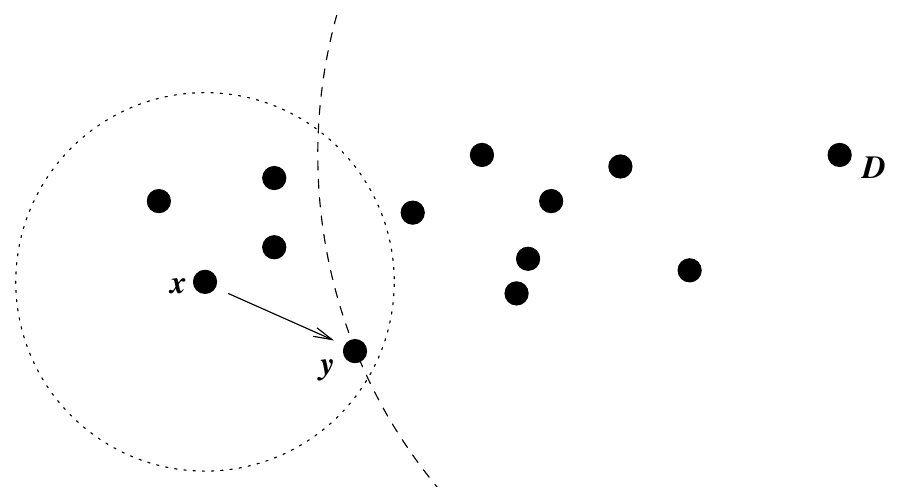
\includegraphics[width=0.55\textwidth]{fig/paper_fig1.png}
\caption[Ví dụ chế độ greedy]{Ví dụ chế độ greedy: $y$ là nút lân cận của $x$ gần $D$ nhất. \src{1}}
\label{fig:greedy}
\end{figure}

Greedy thất bại khi nút đang giữ gói gần đích hơn mọi nút lân cận của nó. Nút đó gọi là \textit{cực đại cục bộ}. Trong Hình~\ref{fig:void}a, $x$ gần $D$ hơn $w$ và $y$, nên greedy dừng ở $x$, dù vẫn có đường $x$ → $y$ → $z$ → $D$. Vùng không có nút nào nằm giữa $x$ và $D$ (vùng tô xám trong Hình~\ref{fig:void}b) gọi là \textit{vùng trống}. Muốn tới đích, gói phải tạm thời đi xa đích hơn để vòng qua vùng trống.

\begin{figure}[H]
\centering
\begin{subfigure}{0.46\textwidth}\centering
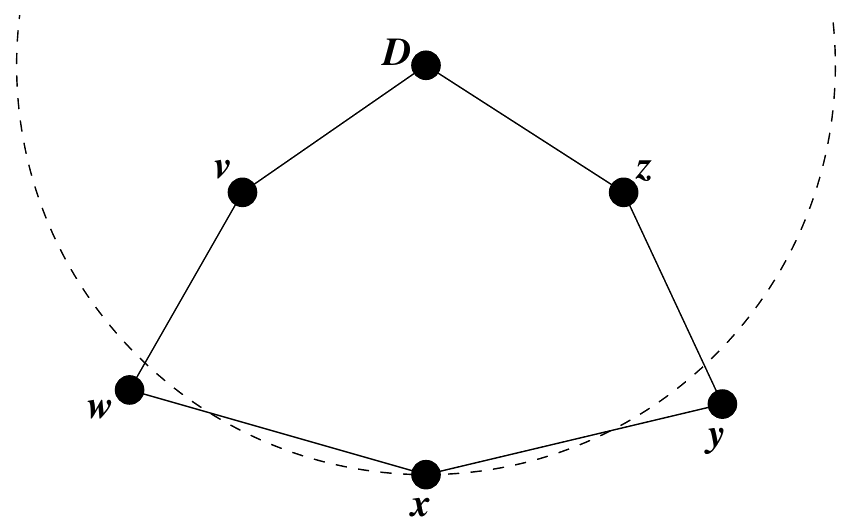
\includegraphics[width=\linewidth]{fig/paper_fig2.png}\caption{$x$ là cực đại cục bộ}
\end{subfigure}\hfill
\begin{subfigure}{0.46\textwidth}\centering
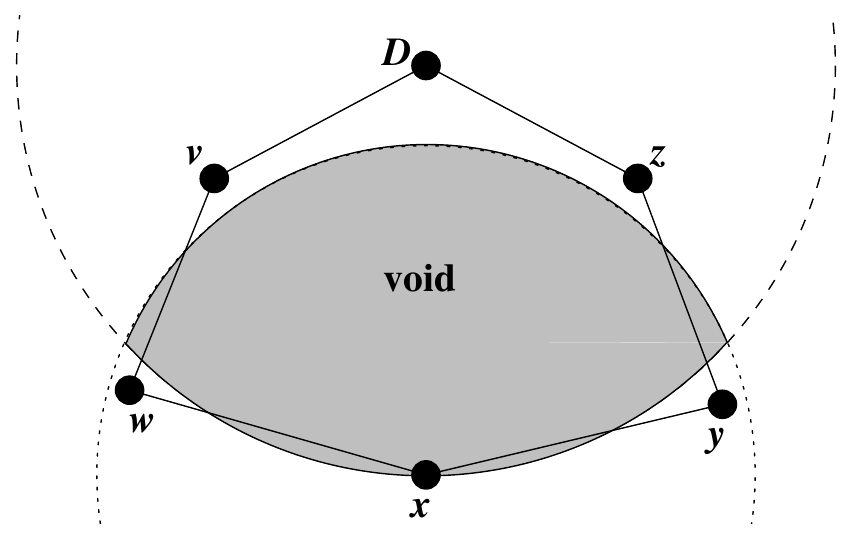
\includegraphics[width=\linewidth]{fig/paper_fig3.png}\caption{Vùng trống của $x$ đối với $D$}
\end{subfigure}
\caption[Greedy thất bại tại cực đại cục bộ]{Greedy thất bại tại cực đại cục bộ. \src{2 và 3}}
\label{fig:void}
\end{figure}

\subsection{Quy tắc bàn tay phải}

Để đi vòng vùng trống, GPSR dùng \textit{quy tắc bàn tay phải}: khi nút $x$ nhận gói từ nút $y$, nó quay ngược chiều kim đồng hồ quanh mình, bắt đầu từ cạnh $(x, y)$, và gửi gói theo cạnh gặp đầu tiên. Lặp lại quy tắc này, gói đi men theo biên của một \textit{mặt}, tức một vùng được bao bởi các cạnh của đồ thị, giống như người đi trong mê cung luôn giữ tay phải chạm tường. Hình~\ref{fig:rhr} minh họa với tam giác $x, y, z$: gói đi lần lượt các cạnh 1, 2, 3.

\begin{figure}[H]
\centering
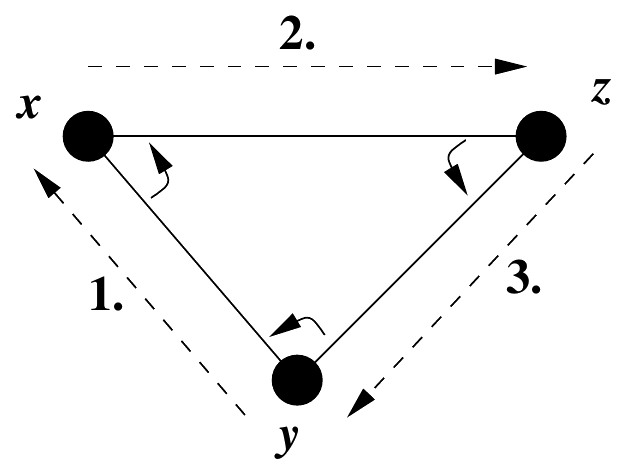
\includegraphics[width=0.42\textwidth]{fig/paper_fig4.png}
\caption[Quy tắc bàn tay phải]{Quy tắc bàn tay phải: $x$ nhận gói từ $y$ và chuyển cho nút lân cận đầu tiên theo chiều ngược kim đồng hồ, là $z$. \src{4}}
\label{fig:rhr}
\end{figure}

\subsection{Làm phẳng đồ thị}

Quy tắc bàn tay phải chỉ đi đúng biên của một mặt khi đồ thị \textit{phẳng}, tức không có hai cạnh nào cắt nhau. Đồ thị các liên kết vô tuyến thường có nhiều cạnh cắt nhau, nên khi chuyển gói ở chế độ perimeter, mỗi nút chỉ dùng một tập con các liên kết của nó. Bài báo đưa ra hai cách chọn tập con, ký hiệu $d(u,v)$ là khoảng cách giữa hai nút $u$ và $v$:

\textbf{RNG.} Giữ cạnh $(u,v)$ nếu không có nút $w$ nào gần cả $u$ và $v$ hơn khoảng cách $d(u,v)$:
\begin{equation}
\forall w \neq u,v:\quad d(u,v) \le \max\left[d(u,w),\, d(v,w)\right]
\end{equation}
Về hình học, vùng giao của hai hình tròn bán kính $d(u,v)$ tâm $u$ và tâm $v$ (vùng xám trong Hình~\ref{fig:planar}a) không được chứa nút nào.

\textbf{GG.} Giữ cạnh $(u,v)$ nếu không có nút $w$ nào nằm trong hình tròn đường kính $uv$ (Hình~\ref{fig:planar}b):
\begin{equation}
\forall w \neq u,v:\quad d^2(u,v) < d^2(u,w) + d^2(v,w)
\end{equation}

\begin{figure}[H]
\centering
\begin{subfigure}{0.4\textwidth}\centering
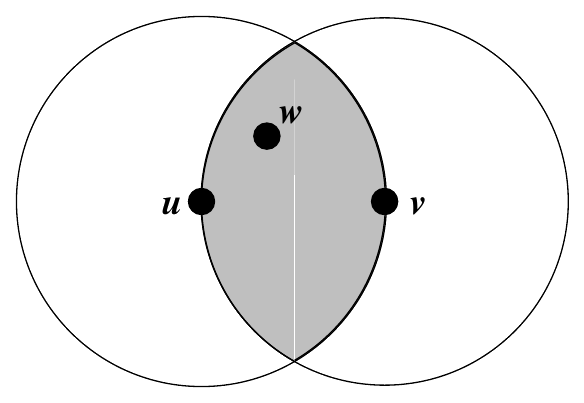
\includegraphics[width=\linewidth]{fig/paper_fig5.png}\caption{RNG}
\end{subfigure}\hspace{1cm}
\begin{subfigure}{0.4\textwidth}\centering
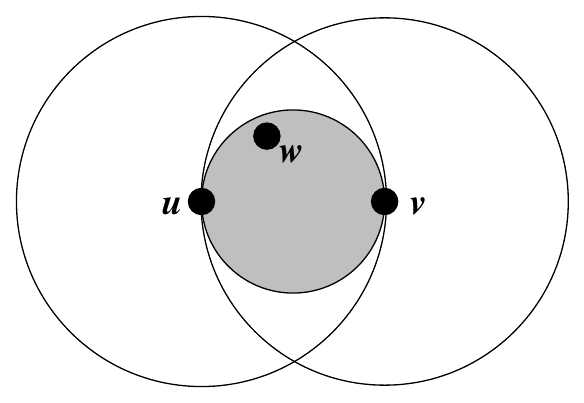
\includegraphics[width=\linewidth]{fig/paper_fig6.png}\caption{GG}
\end{subfigure}
\caption[Điều kiện giữ cạnh của RNG và GG]{Điều kiện giữ cạnh $(u,v)$: vùng xám không được chứa nút $w$ nào. Ở đây có $w$ nên cạnh $(u,v)$ bị bỏ. \src{5 và 6}}
\label{fig:planar}
\end{figure}

Cả hai cách đều chỉ cần vị trí các nút lân cận nên mỗi nút tự tính được. Cả hai cũng giữ được tính liên thông: nếu hai nút có đường đi trong mạng gốc thì vẫn có đường đi trong đồ thị đã làm phẳng. Kết quả mô phỏng của bài báo dùng RNG.

\subsection{Chế độ perimeter}

Khi gặp cực đại cục bộ, gói chuyển sang chế độ perimeter. GPSR ghi thêm vào gói các trường ở Bảng~\ref{tab:hdr}.

\begin{table}[H]
\centering
\caption{Các trường GPSR ghi trong gói}
\label{tab:hdr}
\begin{tabularx}{0.85\textwidth}{>{\centering\arraybackslash}p{1.4cm} L}
\toprule
Trường & Ý nghĩa\\
\midrule
$D$ & Vị trí của đích\\
$L_p$ & Vị trí nơi gói bắt đầu vào chế độ perimeter\\
$L_f$ & Điểm trên đoạn thẳng $L_pD$ nơi gói bắt đầu đi trên mặt hiện tại\\
$e_0$ & Cạnh đầu tiên gói đi trên mặt hiện tại\\
$M$ & Chế độ hiện tại: greedy hoặc perimeter\\
\bottomrule
\end{tabularx}
\end{table}

Quá trình chuyển gói ở chế độ perimeter như sau:
\begin{enumerate}[leftmargin=1.6cm]
  \item \textbf{Chặng đầu tiên:} Tại $L_p$, gói đi theo cạnh đầu tiên ngược chiều kim đồng hồ tính từ đoạn thẳng nối $L_p$ với $D$.
  \item \textbf{Các chặng sau:} Gói đi theo quy tắc bàn tay phải trên đồ thị đã làm phẳng.
  \item \textbf{Đổi mặt:} Nếu cạnh sắp đi cắt đoạn $L_pD$ tại một điểm gần $D$ hơn $L_f$, gói chuyển sang mặt kế tiếp nằm trên đoạn thẳng đó và cập nhật $L_f$, $e_0$.
  \item \textbf{Quay lại greedy:} Ngay khi gói tới một nút gần $D$ hơn $L_p$.
  \item \textbf{Bỏ gói:} Nếu gói đi lại đúng cạnh $e_0$, tức đã đi hết một vòng của mặt mà không tiến được, thì đích không thể tới.
\end{enumerate}

Hình~\ref{fig:perim} là ví dụ gói đi từ $x$ tới $D$: gói lần lượt đi qua các mặt bị đoạn thẳng $xD$ (nét đứt) cắt qua, mỗi mặt gần $D$ hơn mặt trước.

\begin{figure}[H]
\centering
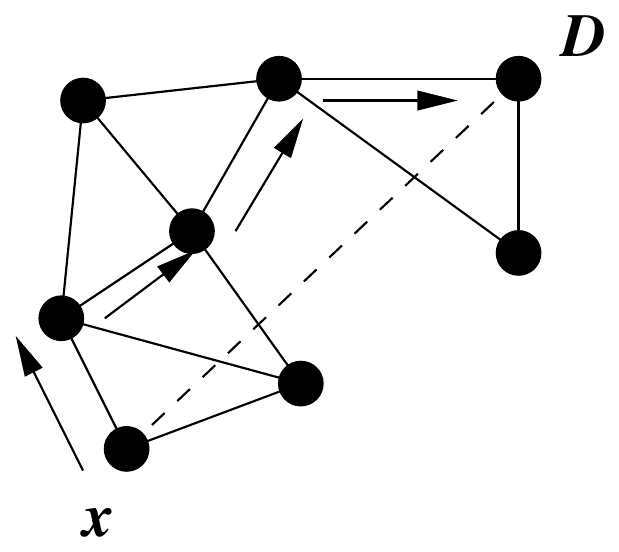
\includegraphics[width=0.45\textwidth]{fig/paper_fig8.png}
\caption[Ví dụ chế độ perimeter]{Ví dụ chế độ perimeter: gói đi qua các mặt bị đoạn $xD$ cắt qua. \src{8}}
\label{fig:perim}
\end{figure}

\subsection{Phản hồi lỗi từ tầng MAC}

Bảng nút lân cận có thể cũ: một nút vẫn nằm trong bảng dù đã ra khỏi tầm sóng. Khi gửi tới nút đó, 802.11 gửi lại khung nhiều lần rồi báo thất bại lên tầng trên. Mục 2.5 của bài báo nêu hai cách GPSR dùng báo lỗi này:
\begin{itemize}
  \item \textbf{Xóa nút lân cận:} Báo lỗi được xử lý như khi nút đó hết hạn trong bảng, nên GPSR biết nút đã đi xa sớm hơn so với chờ hết $4{,}5B$.
  \item \textbf{Duyệt hàng đợi:} GPSR lấy ra mọi gói đang chờ gửi tới nút đó trong hàng đợi của card mạng và chuyển tiếp lại chúng qua nút lân cận khác. Nếu không làm vậy, card mạng lần lượt gửi thử từng gói tới một nút đã đi mất và bị chặn trong thời gian dài. Theo tác giả, chi tiết này ảnh hưởng rất lớn tới kết quả.
\end{itemize}
Bài báo không nói rõ gói vừa gửi lỗi có được gửi lại hay không. Bản cài đặt của báo cáo gửi lại gói đó cùng với các gói trong hàng đợi.

\section{Kết quả bài báo đã công bố}

Bài báo mô phỏng GPSR trên ns-2 trong mạng 50, 112 và 200 nút di chuyển ngẫu nhiên, so sánh với DSR. Bảng~\ref{tab:paper} tóm tắt các kết quả cần tái hiện.

\begin{table}[H]
\centering
\caption{Các kết quả chính của bài báo}
\label{tab:paper}
\begin{tabularx}{\textwidth}{>{\raggedright\arraybackslash}p{4.2cm} >{\centering\arraybackslash}p{2.2cm} L}
\toprule
Kết quả & Trong bài báo & Nội dung\\
\midrule
PDR, 50 nút & Hình 9 & Trên 97\% với mọi $B$; $B = 3$\,s thấp hơn $B = 1$ và $1{,}5$\,s\\
Số gói điều khiển, 50 nút & Hình 10 & Không đổi theo mức di chuyển, tỉ lệ nghịch với $B$, thấp hơn DSR\\
Độ dài đường đi & Hình 11 & 97\% gói đi đúng số chặng ngắn nhất\\
PDR, 112 và 200 nút & Hình 12 & Vẫn cao (khoảng 94--99\%) khi mạng lớn lên\\
Số gói điều khiển, 112 và 200 nút & Hình 13 & Không đổi theo mức di chuyển, tăng theo số nút\\
Số nút mỗi nút phải lưu & Mục 3.6 & Trung bình 26 nút (200 nút, pause 0)\\
\bottomrule
\end{tabularx}
\end{table}

% ============================ CHƯƠNG 2 =====================================
\chapter{Cài đặt trên ns-3 và kịch bản mô phỏng}

Bài báo không kèm mã nguồn cho ns-3, nên GPSR được cài đặt thành một module riêng của ns-3.43, đóng vai trò giao thức định tuyến của tầng IPv4.

\section{Các thành phần cài đặt}

Bảng~\ref{tab:modules} liệt kê các thành phần chính và phần thuật toán mà mỗi thành phần đảm nhận.

\begin{table}[H]
\centering
\caption{Các thành phần cài đặt GPSR}
\label{tab:modules}
\small
\begin{tabularx}{\textwidth}{>{\raggedright\arraybackslash}p{3.6cm} L >{\centering\arraybackslash}p{1.8cm}}
\toprule
Thành phần & Chức năng & Mục\\
\midrule
\texttt{HelloHeader} & Gói beacon 8 byte chứa tọa độ $x$, $y$; phát theo chu kỳ ngẫu nhiên trong $[0{,}5B;\ 1{,}5B]$ & 1.3.1\\
\texttt{PositionTable} & Bảng nút lân cận: thêm, xóa sau $4{,}5B$; chọn nút gần đích nhất; kiểm tra cạnh RNG/GG; chọn cạnh theo quy tắc bàn tay phải & 1.3.1--1.3.5\\
\texttt{PerimeterTag} & Các trường ở Bảng~\ref{tab:hdr} và số chặng, gắn theo từng gói & 1.3.5\\
\texttt{RoutingProtocol} & Nhận gói từ tầng IP, chọn chặng tiếp theo theo greedy hoặc perimeter; nghe lén gói dữ liệu; hoãn beacon khi vừa gửi dữ liệu & 1.3.1--1.3.5\\
Xử lý lỗi MAC & Nhận báo lỗi khi 802.11 gửi lại quá số lần, xóa nút lân cận đó, chuyển tiếp lại gói lỗi và mọi gói trong hàng đợi gửi tới nút đó & 1.3.6\\
\texttt{GpsrHelper} & Cài GPSR lên các nút; tham số $B$ và cách làm phẳng (RNG hoặc GG) & --\\
\texttt{gpsr-paper-scenario} & Kịch bản mô phỏng theo mục 3 của bài báo và các phép đo & --\\
\texttt{gpsr-void-test} & Kiểm thử chế độ perimeter (mục 3.1) & --\\
\texttt{run\_sim\_and\_plot.py} & Chạy song song các lần mô phỏng, tính trung bình và vẽ đồ thị & --\\
\bottomrule
\end{tabularx}
\end{table}

Vị trí đích được lấy trực tiếp từ mô hình di chuyển của nút đích tại thời điểm gửi. Bài báo cũng giả định như vậy: nguồn luôn biết vị trí thật của đích, và dịch vụ tra cứu vị trí không được mô phỏng.

\section{Kịch bản mô phỏng}

Các tham số trong Bảng~\ref{tab:params} được giữ đúng như mục 3.1 của bài báo.

\begin{table}[H]
\centering
\caption{Tham số mô phỏng}
\label{tab:params}
\begin{tabularx}{\textwidth}{>{\raggedright\arraybackslash}p{4.2cm} L}
\toprule
Tham số & Giá trị\\
\midrule
Số nút và vùng mô phỏng & 50 nút -- 1500 × 300\,m; 112 nút -- 2250 × 450\,m; 200 nút -- 3000 × 600\,m (cùng mật độ 1 nút / 9000\,m$^2$)\\
Tầng MAC và vô tuyến & IEEE 802.11, 2\,Mbit/s, tầm sóng 250\,m\\
Di chuyển & Random waypoint: nút đi tới một điểm ngẫu nhiên với vận tốc ngẫu nhiên tối đa 20\,m/s, dừng lại trong khoảng \textit{pause time}, rồi lặp lại\\
Pause time & 0, 30, 60, 120\,s (pause càng nhỏ, nút càng di chuyển nhiều)\\
Lưu lượng & 30 luồng CBR do 22 nút gửi, gói 64 byte, 2\,Kbit/s mỗi luồng (4 gói/s)\\
Thời gian mô phỏng & 900\,s\\
Chu kỳ beacon $B$ & 1; 1,5; 3\,s (mạng 50 nút); 1,5\,s (mạng 112 và 200 nút)\\
Làm phẳng & RNG\\
Số lần chạy & 6 lần mỗi cấu hình, mỗi lần một kịch bản di chuyển khác nhau\\
\bottomrule
\end{tabularx}
\end{table}

Một số chi tiết bài báo không nêu, hoặc được báo cáo chọn khác đi, như sau:
\begin{itemize}
  \item \textbf{Kênh vô tuyến:} Bài báo dùng mô hình two-ray ground của ns-2. Báo cáo dùng mô hình \texttt{RangePropagationLossModel} của ns-3 để tầm sóng đúng bằng 250\,m: trong phạm vi này, khung tin luôn nhận được nếu không bị va chạm; ngoài 250\,m, nút hoàn toàn không nghe thấy tín hiệu. ns-3 cũng có mô hình two-ray ground, nhưng muốn dùng nó phải chỉnh thêm ngưỡng thu và ngưỡng nghe sóng cho khớp ns-2, mà bài báo không cung cấp các ngưỡng này.
  \item \textbf{Vận tốc tối thiểu 1\,m/s:} Tránh trường hợp nút chọn vận tốc gần 0 và gần như đứng yên cả lần mô phỏng.
  \item \textbf{Thời điểm bắt đầu mỗi luồng:} Ngẫu nhiên trong khoảng 10--100\,s, để các nút kịp trao đổi beacon trước.
  \item \textbf{Tắt RTS/CTS.}
\end{itemize}

Tổng số lần chạy là 102: 72 lần cho mạng 50 nút (3 giá trị $B$ × 4 pause time × 6), 24 lần cho mạng 112 nút (4 pause time × 6) và 6 lần cho mạng 200 nút (chỉ pause 0, như bài báo).

\section{Khác biệt so với môi trường của bài báo}

Bài báo chạy trên ns-2 với mã GPSR của chính tác giả; báo cáo chạy trên ns-3.43 với mã viết mới theo mô tả trong bài. Bảng~\ref{tab:diff} liệt kê các khác biệt có thể ảnh hưởng tới kết quả. Chương~5 dùng bảng này để giải thích các chênh lệch.

\begin{table}[H]
\centering
\caption{Khác biệt giữa môi trường của bài báo và của báo cáo}
\label{tab:diff}
\small
\begin{tabularx}{\textwidth}{>{\raggedright\arraybackslash}p{2.6cm} L L L}
\toprule
Yếu tố & Bài báo (ns-2) & Báo cáo (ns-3.43) & Ảnh hưởng dự kiến\\
\midrule
Mã GPSR & Bản của tác giả & Viết mới theo mô tả trong bài & Phải kiểm chứng lại hành vi (Chương 3)\\
Kênh vô tuyến & Mô hình two-ray ground, nhận được trong 250\,m; theo cấu hình mặc định của ns-2 (bài báo không nêu), tín hiệu tới khoảng 550\,m vẫn gây nhiễu & Nhận được trong 250\,m; ngoài 250\,m không có tín hiệu & Ít nhiễu và va chạm hơn, PDR có thể cao hơn\\
ARP & ARP động & Bảng ARP tĩnh & Không mất gói vì ARP (xem dưới)\\
RTS/CTS & Không nêu & Tắt & --\\
Vận tốc nút & Tối đa 20\,m/s & 1--20\,m/s & Không đáng kể\\
Bắt đầu luồng & Không nêu & Ngẫu nhiên 10--100\,s & --\\
Giao thức đối chứng & DSR của CMU & Không chạy lại (mục 2.4) & So với số liệu DSR trong bài\\
\bottomrule
\end{tabularx}
\end{table}

Thay đổi quan trọng nhất là ARP, giao thức tìm địa chỉ MAC của một nút từ địa chỉ IP. Lần chạy đầu tiên của báo cáo dùng ARP động mặc định của ns-3 và cho PDR thấp hơn bài báo rất nhiều (kết quả này được so với bản cuối ở mục 5.3). Khi đếm nguyên nhân mất gói trong một lần chạy 50 nút, $B = 3$\,s, pause 0, 300\,s, 88\% số gói mất là do ARP. Cơ chế gây mất gói như sau:
\begin{enumerate}[leftmargin=1.6cm]
  \item GPSR chọn một nút lân cận đã đi khỏi tầm nhưng còn trong bảng.
  \item Yêu cầu ARP tới nút đó không được trả lời, gói bị bỏ ngay tại ARP và tầng MAC không báo lỗi.
  \item Không có báo lỗi nên GPSR không xóa nút đó khỏi bảng, các gói sau tiếp tục bị gửi tới nó.
  \item Trình mô phỏng ns-3 còn đánh dấu địa chỉ đó là không dùng được trong 100\,s và bỏ mọi gói gửi tới nó, kể cả khi nút đã quay lại tầm.
\end{enumerate}
Như vậy, ARP động của ns-3 vô hiệu hóa cơ chế phản hồi lỗi MAC ở mục 1.3.6. Bảng ARP tĩnh nạp sẵn địa chỉ MAC của mọi nút từ đầu mô phỏng, nên mọi lần gửi đều đi qua tầng MAC và được cơ chế đó xử lý.

\section{Không mô phỏng lại DSR}

Bài báo dùng DSR làm giao thức đối chứng, với bản cài đặt của nhóm CMU trên ns-2 [2]. Trình mô phỏng ns-3 có module DSR riêng, là một bản cài đặt khác. Báo cáo đã chạy thử module này với mạng 50 nút: PDR chỉ đạt 54--73\% và số gói điều khiển khoảng 90.000--180.000, trong khi bài báo cho DSR khoảng 97--98\% và 27.000--41.000 gói. Với chênh lệch lớn như vậy, DSR trong ns-3 không đại diện được cho DSR trong bài báo, và so GPSR với nó sẽ dẫn tới kết luận sai. Mỗi lần chạy DSR cũng chậm hơn GPSR nhiều lần vì số gói điều khiển lớn.

Vì vậy báo cáo chỉ chạy GPSR. Khi cần so với DSR, báo cáo dùng số liệu DSR đã công bố trong bài báo (đường chấm trong Hình~4.2).

\section{Các đại lượng đo}

\begin{itemize}
  \item \textbf{Tỉ lệ gửi gói thành công (PDR):} Như bài báo, chỉ tính những gói mà lúc gửi có tồn tại đường đi tới đích:
  \begin{equation}
  \text{PDR} = \frac{\text{số gói tới đích}}{\text{số gói gửi khi nguồn và đích còn đường đi}}
  \end{equation}
  Đường đi được kiểm tra bằng tìm kiếm theo chiều rộng trên vị trí thật của các nút; hai nút cách nhau không quá 250\,m thì có liên kết.
  \item \textbf{Số gói điều khiển (overhead):} Tổng số beacon mọi nút đã phát trong 900\,s.
  \item \textbf{Độ dài đường đi so với tối ưu:} Với mỗi gói tới đích, lấy số chặng thực tế trừ số chặng của đường ngắn nhất tại lúc gửi (mạng 50 nút, $B = 1{,}5$\,s, pause 0, như Hình 11 của bài báo).
  \item \textbf{Số nút lân cận trong bảng:} Trung bình trên mọi nút, lấy tại giây 300 (như mục 3.6 của bài báo).
\end{itemize}

Mỗi giá trị trong báo cáo là trung bình của 6 lần chạy.

% ============================ CHƯƠNG 3 =====================================
\chapter{Kiểm tra tính đúng đắn}

Bốn kiểm thử trong Bảng~\ref{tab:tests} kiểm tra từng phần của thuật toán trước khi chạy thí nghiệm chính. Cả bốn đều đạt.

\begin{table}[H]
\centering
\caption{Các kiểm thử và kết quả}
\label{tab:tests}
\small
\begin{tabularx}{\textwidth}{>{\raggedright\arraybackslash}p{3cm} >{\raggedright\arraybackslash}p{3.1cm} L L}
\toprule
Kiểm thử & Phần được kiểm tra & Kết quả mong đợi & Kết quả đo\\
\midrule
3.1. Topo có vùng trống & Perimeter, RNG và GG & Mọi gói tới đích, đi đúng 7 chặng & RNG và GG: 196/196 gói, đều 7 chặng\\
3.2. Mạng tĩnh 50 nút & Greedy và perimeter trên topo ngẫu nhiên & PDR 100\% & 100\% ở cả 3 kịch bản\\
3.3. Mạng di động 50 nút & Phản hồi lỗi MAC & Lỗi MAC nhiều nhưng gói vẫn tới đích & 6.193 lần lỗi MAC, PDR 99,985\%\\
3.4. Đếm beacon & Beacon và cơ chế hoãn beacon & Nhỏ hơn cận trên $NT/B$ & 32--35\% cận trên với cả 3 giá trị $B$\\
\bottomrule
\end{tabularx}
\end{table}

\section{Chế độ perimeter trên topo có vùng trống}

Tám nút đứng yên được đặt như Hình~\ref{fig:voidtest}, tầm sóng 250\,m. Nguồn $S$ gửi 4 gói/s tới đích $D$ trong khoảng 50\,s. Nút $A$ gần $D$ hơn mọi nút lân cận của nó ($S$ và $B$), nên greedy chắc chắn dừng ở $A$. Gói chỉ tới được $D$ nếu chế độ perimeter đưa nó từ $A$ qua $B$ tới $C$. Tại $C$, khoảng cách tới $D$ là 671\,m, nhỏ hơn 800\,m của $A$, nên gói quay lại greedy và đi tiếp $E$--$F$--$G$--$D$. Đường duy nhất từ $S$ tới $D$ dài 7 chặng.

\begin{figure}[H]
\centering
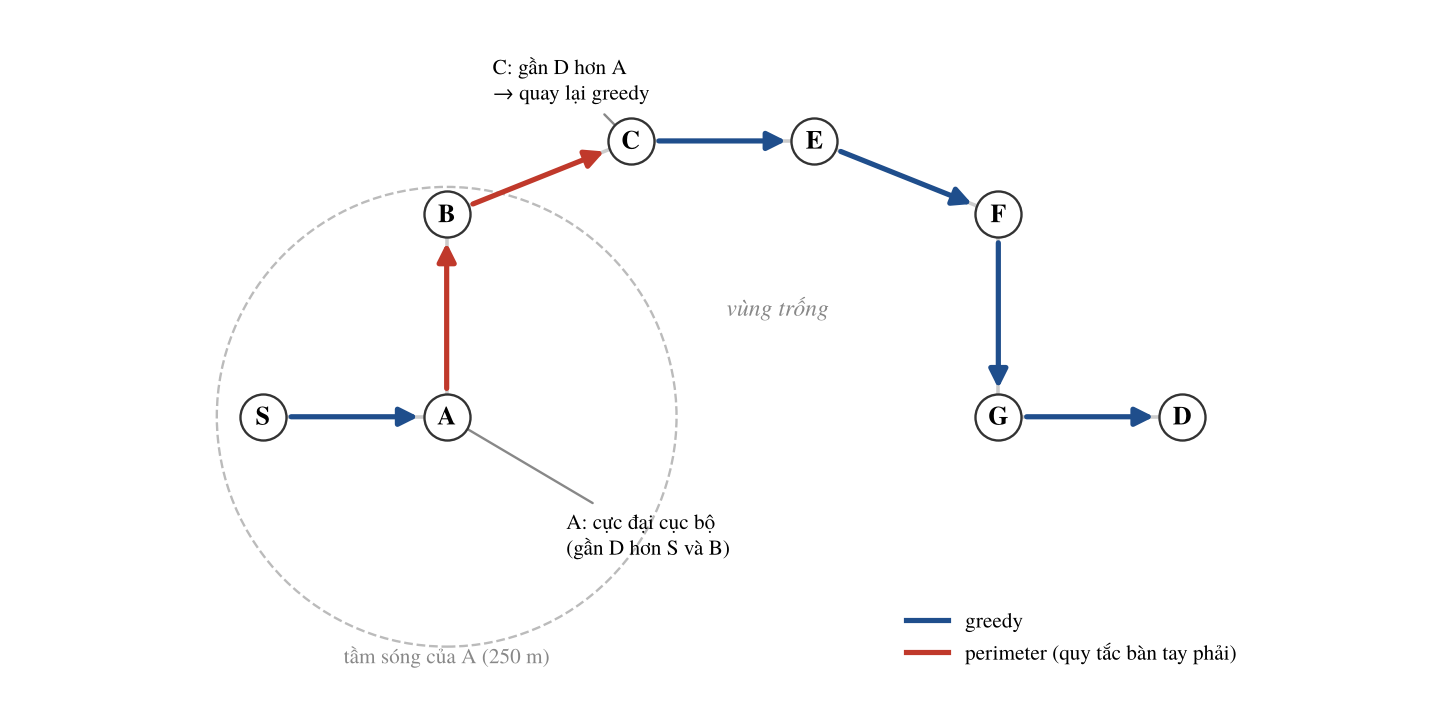
\includegraphics[width=0.85\textwidth]{fig/h1_1.png}
\caption{Topo kiểm thử chế độ perimeter}
\label{fig:voidtest}
\end{figure}

Kết quả: Với cả RNG và GG, 196/196 gói tới $D$ và gói nào cũng đi đúng 7 chặng. Vậy chế độ perimeter và việc quay lại greedy hoạt động đúng, gói không đi thừa chặng nào.

\section{Mạng tĩnh 50 nút}

Bài báo kiểm tra cài đặt của mình bằng cách chạy trên các topo không di chuyển, với mục tiêu giao 100\% gói. Khi nút đứng yên, bảng nút lân cận luôn đúng, nên mỗi gói bị mất đều chỉ ra một lỗi trong quyết định chọn đường.

Báo cáo làm tương tự: 50 nút đặt ngẫu nhiên và đứng yên (pause time bằng thời gian mô phỏng), lưu lượng như thí nghiệm chính, 300\,s, với 3 cách đặt nút khác nhau. Số gói tới đích lần lượt là 29.900/29.900, 29.798/29.798 và 28.914/28.914, tức PDR 100\%.

\section{Phản hồi lỗi MAC trong mạng di động}

Khi nút di chuyển, bảng nút lân cận có lúc cũ và 802.11 sẽ báo lỗi khi gửi tới nút đã đi xa. Ở một lần chạy 50 nút, $B = 1{,}5$\,s, pause 0, 900\,s, tầng MAC báo lỗi 6.193 lần. Nếu mỗi lỗi làm mất một gói, PDR sẽ giảm khoảng 6 điểm phần trăm. PDR đo được là 99,985\% (101.584/101.599 gói), nghĩa là gần như mọi gói gặp lỗi đều được chuyển lại qua nút khác.

\section{Số beacon}

Nếu không hoãn beacon, $N$ nút trong $T$ giây phát khoảng $N T / B$ beacon. Với 50 nút và 900\,s, cận trên này là 45.000 ($B = 1$\,s), 30.000 ($B = 1{,}5$\,s) và 15.000 ($B = 3$\,s).

Số đo trung bình ở pause 0 là 15.784, 10.273 và 4.807, tức 35\%, 34\% và 32\% cận trên. Phần giảm đi đến từ các nút đang gửi hoặc chuyển tiếp dữ liệu, vốn không cần phát beacon. Tỉ lệ gần như nhau với cả 3 giá trị $B$, đúng với việc số beacon tỉ lệ nghịch với $B$.

% ============================ CHƯƠNG 4 =====================================
\chapter{Kết quả thí nghiệm}

Các thí nghiệm chạy với kịch bản ở mục 2.2. Mỗi hình dưới đây tương ứng một hình của bài báo. Đường nét liền là kết quả ns-3 (trung bình 6 lần chạy, thanh sai số là độ lệch chuẩn); đường nét đứt là số liệu bài báo, đọc từ đồ thị gốc nên chỉ là xấp xỉ.

\section{Tỉ lệ gửi gói thành công, mạng 50 nút}

Hình~\ref{fig:r1} (tương ứng Hình 9 của bài báo) cho biết tỉ lệ gói tới đích khi nút di chuyển nhiều (pause 0) hay ít (pause 120\,s), với 3 chu kỳ beacon.

\begin{figure}[H]
\centering
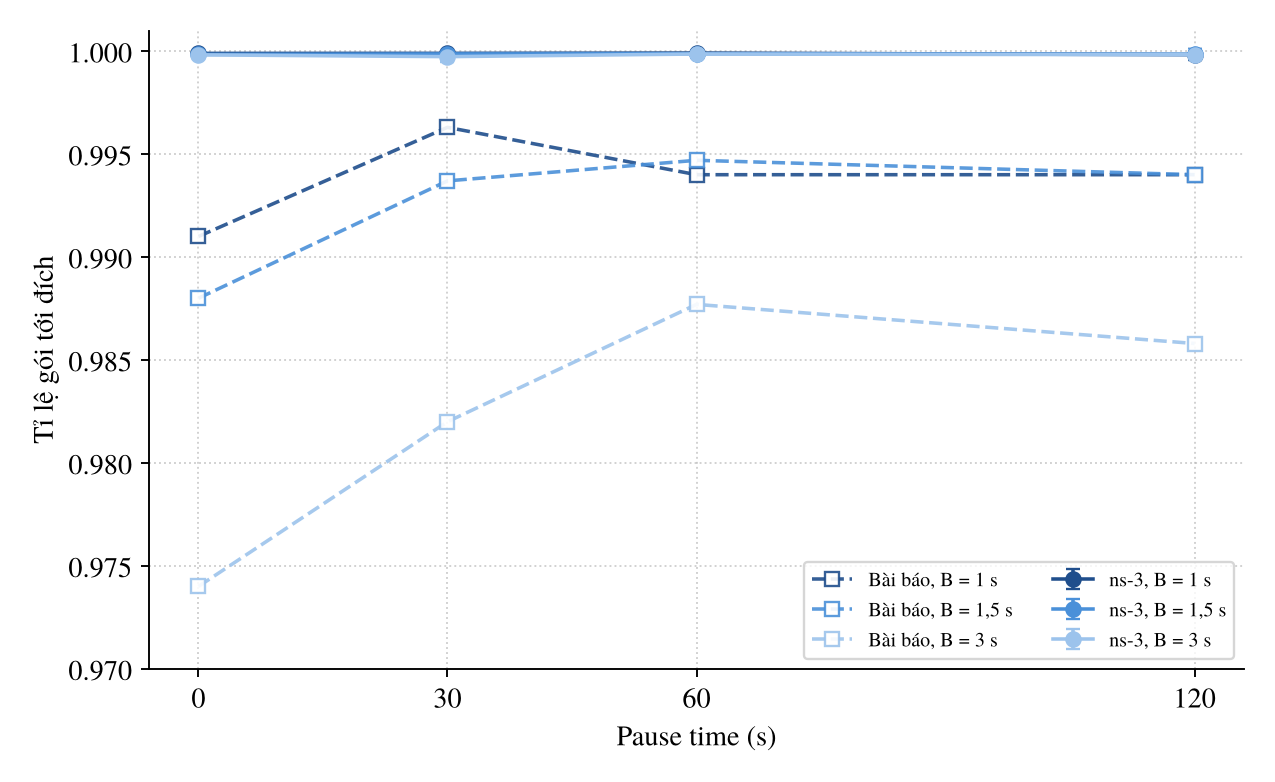
\includegraphics[width=0.78\textwidth]{fig/h4_1.png}
\caption{PDR theo pause time, 50 nút}
\label{fig:r1}
\end{figure}

PDR trong ns-3 nằm trong khoảng 99,97--99,99\% ở cả 12 cấu hình, các đường gần như trùng nhau ở sát mức 1. Bài báo cho 97,4--99,6\%: $B = 3$\,s thấp rõ rệt hơn hai giá trị còn lại, và PDR tăng khi nút ít di chuyển hơn. Trong ns-3, cả hai xu hướng đó đều nhỏ hơn sai số giữa các lần chạy.

\section{Số gói điều khiển, mạng 50 nút}

Hình~\ref{fig:r2} (tương ứng Hình 10) cho biết tổng số beacon cả mạng phát trong 900\,s.

\begin{figure}[H]
\centering
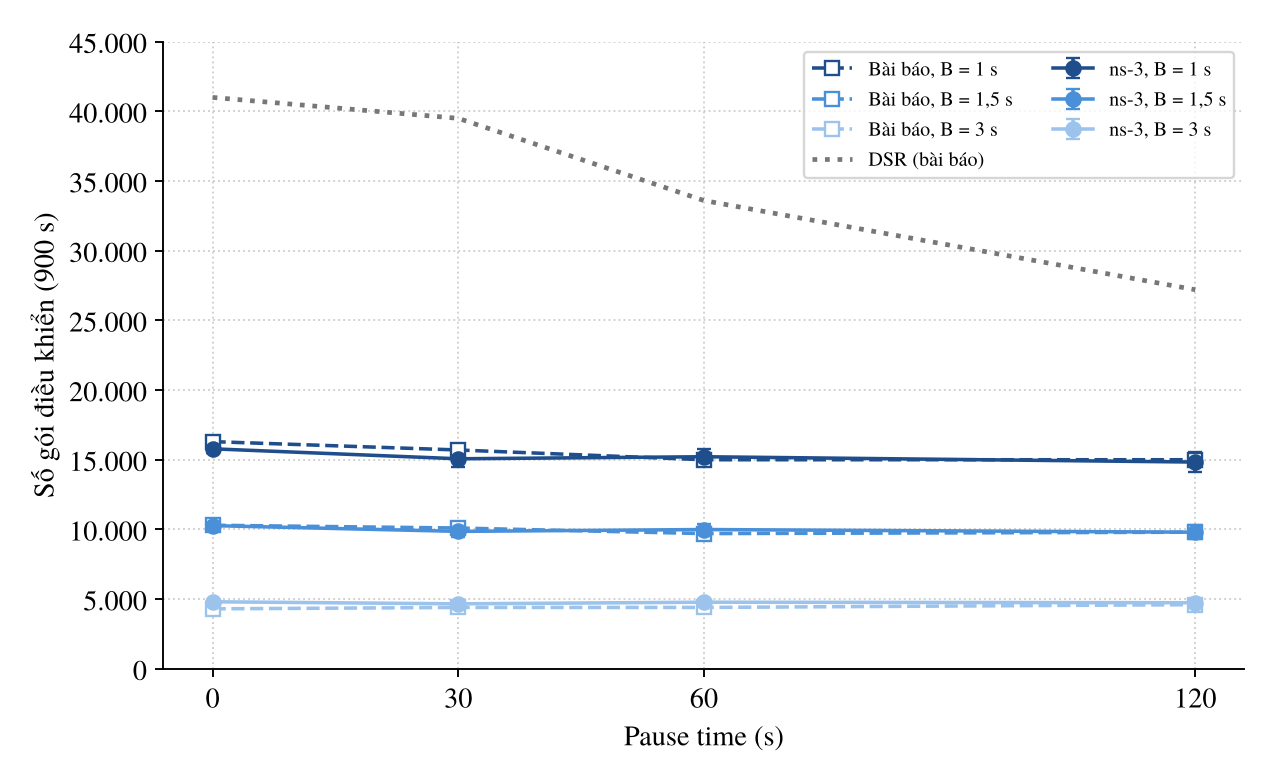
\includegraphics[width=0.78\textwidth]{fig/h4_2.png}
\caption[Số gói điều khiển theo pause time, 50 nút]{Số gói điều khiển theo pause time, 50 nút. Đường chấm là DSR trong bài báo, để tham chiếu.}
\label{fig:r2}
\end{figure}

Số gói điều khiển gần như không đổi theo pause time: khoảng 15.000 gói với $B = 1$\,s, 10.000 với $B = 1{,}5$\,s và 4.700 với $B = 3$\,s. Lý do là beacon được phát theo chu kỳ cố định, dù nút di chuyển nhiều hay ít. Cả ba đường gần như trùng với bài báo, và đều nằm dưới DSR trong bài báo (27.000--41.000 gói).

\section{Độ dài đường đi so với tối ưu}

Hình~\ref{fig:r3} (tương ứng Hình 11) chia các gói đã tới đích theo số chặng đi thừa so với đường ngắn nhất (50 nút, $B = 1{,}5$\,s, pause 0).

\begin{figure}[H]
\centering
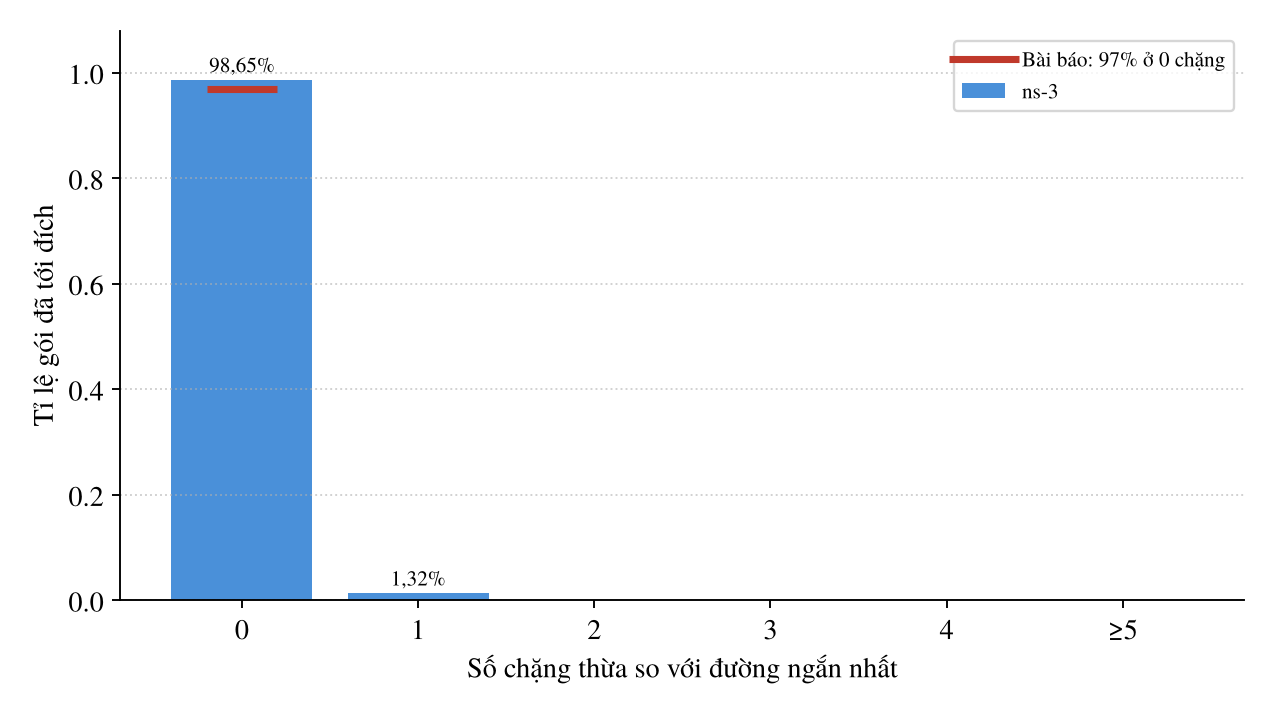
\includegraphics[width=0.8\textwidth]{fig/h4_3.png}
\caption{Phân bố số chặng thừa so với đường ngắn nhất}
\label{fig:r3}
\end{figure}

98,65\% gói đi đúng số chặng ngắn nhất, 1,32\% đi thừa một chặng, gần như không gói nào thừa từ hai chặng trở lên. Bài báo cho 97\%. Mạng dày đặc (khoảng 20 nút lân cận) nên greedy gần như luôn tìm được bước tiến tốt nhất.

\section{Tỉ lệ gửi gói thành công khi mạng lớn hơn}

Hình~\ref{fig:r4} (tương ứng Hình 12) so sánh mạng 50, 112 và 200 nút với cùng mật độ nút, $B = 1{,}5$\,s. Mạng lớn hơn thì đường đi dài hơn: trung bình 2,3 chặng (50 nút), 3,5 chặng (112 nút) và 4,4 chặng (200 nút) ở pause 0.

\begin{figure}[H]
\centering
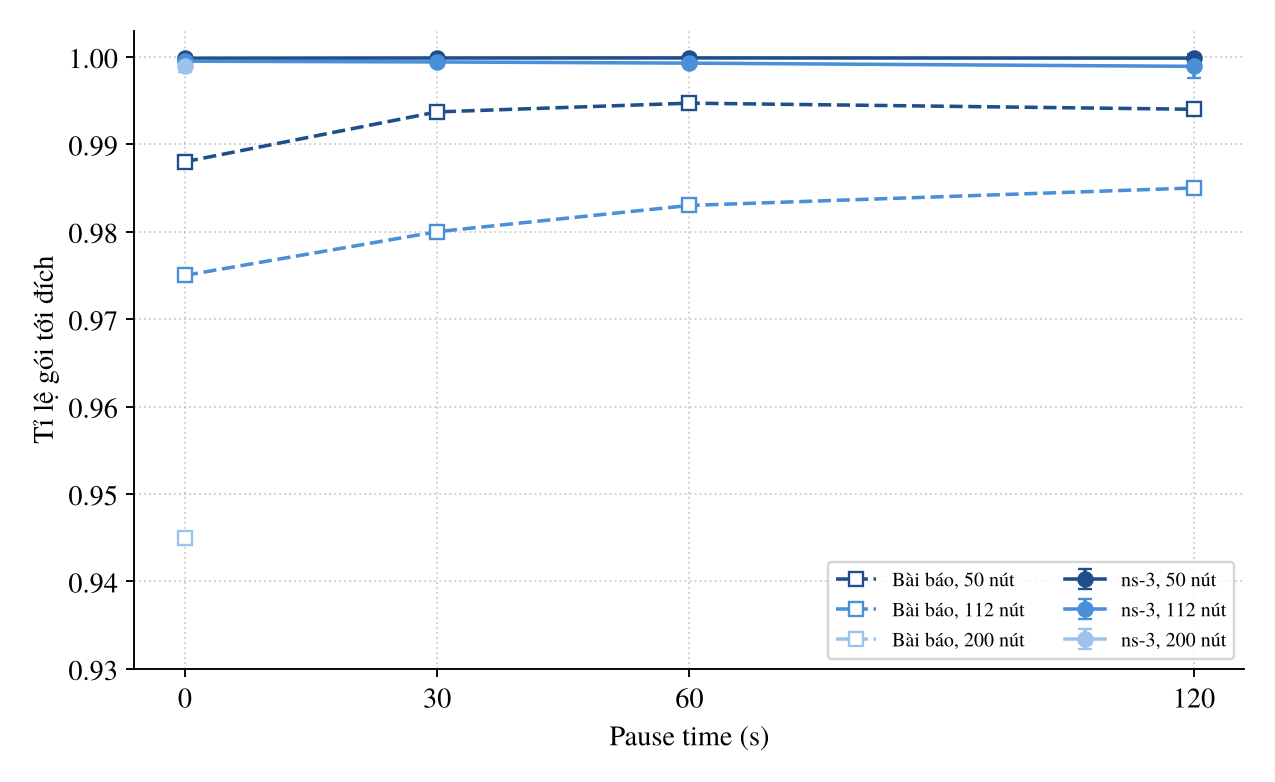
\includegraphics[width=0.78\textwidth]{fig/h4_4.png}
\caption[PDR theo số nút]{PDR theo số nút, $B = 1{,}5$\,s (mạng 200 nút chỉ chạy pause 0, như bài báo)}
\label{fig:r4}
\end{figure}

PDR giảm rất nhẹ khi mạng lớn lên: 99,98--99,99\% (50 nút), 99,89--99,95\% (112 nút), 99,90\% (200 nút). Bài báo cũng cho xu hướng giảm nhưng mạnh hơn: khoảng 97,5--98,5\% (112 nút) và 94,5\% (200 nút). Gói đi càng nhiều chặng thì càng có nhiều cơ hội bị mất.

\section{Số gói điều khiển khi mạng lớn hơn}

Hình~\ref{fig:r5} tương ứng Hình 13 của bài báo, trục dọc theo thang logarit.

\begin{figure}[H]
\centering
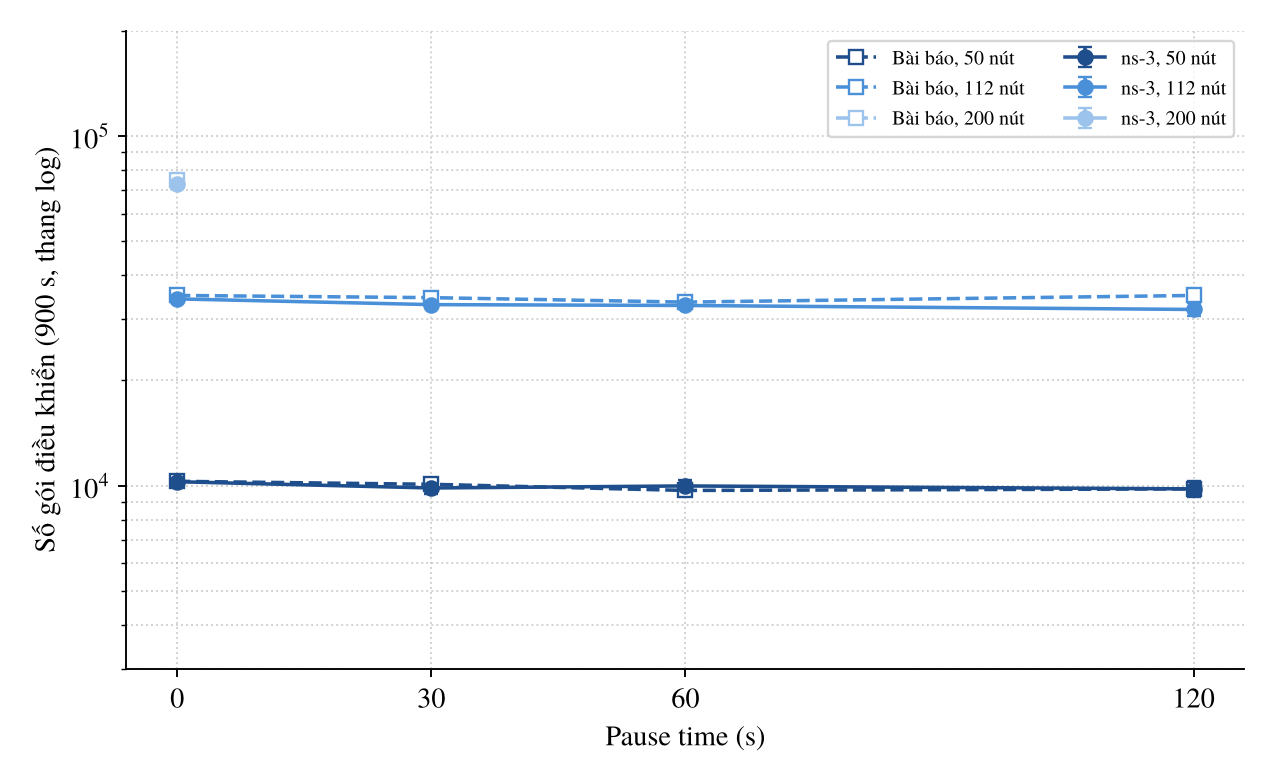
\includegraphics[width=0.78\textwidth]{fig/h4_5.png}
\caption{Số gói điều khiển theo số nút, $B = 1{,}5$\,s}
\label{fig:r5}
\end{figure}

Số gói điều khiển là khoảng 10.000 (50 nút), 32.000--34.000 (112 nút) và 72.800 (200 nút), và gần như không đổi theo pause time. Con số tăng theo số nút vì có nhiều nút phát beacon hơn; mỗi beacon chỉ đi một chặng, nên đường kính mạng không ảnh hưởng. Số liệu bài báo là khoảng 34.000 và 75.000.

\section{Số nút lân cận mỗi nút phải lưu}

Tại giây 300, mỗi nút trong mạng 200 nút, pause 0 lưu trung bình 28,6 nút lân cận; bài báo cho 26. Theo bài báo, số này do mật độ nút quyết định, không do tổng số nút. Trong ns-3, số này vẫn tăng nhẹ theo kích thước mạng: khoảng 18, 25 và 29 ở mạng 50, 112 và 200 nút (pause 0). Lý do là vùng mô phỏng của mạng nhỏ hẹp hơn (chỉ rộng 300\,m ở mạng 50 nút), nên tỉ lệ nút nằm sát biên, có ít nút lân cận, lớn hơn.

% ============================ CHƯƠNG 5 =====================================
\chapter{So sánh với bài báo và nhận xét}

Các đại lượng chỉ phụ thuộc thuật toán (số gói điều khiển, độ dài đường đi, số nút lân cận) khớp bài báo, kể cả ở những chi tiết nhỏ. PDR cao hơn bài báo và không còn thể hiện ảnh hưởng của $B$ và pause time. Bảng~\ref{tab:cmp} tổng hợp; số liệu bài báo đọc từ đồ thị nên chỉ là xấp xỉ.

\begin{table}[H]
\centering
\caption{So sánh kết quả ns-3 với bài báo}
\label{tab:cmp}
\small
\begin{tabularx}{\textwidth}{>{\raggedright\arraybackslash}p{5.1cm} L L >{\raggedright\arraybackslash}p{2.9cm}}
\toprule
Kết quả & Bài báo & ns-3 & Chênh lệch\\
\midrule
Gói điều khiển, 50 nút, \textit{B} = 1 s & ≈ 15.000--16.300 & 14.834--15.784 & −4\% đến +1\%\\
Gói điều khiển, 50 nút, \textit{B} = 1,5 s & ≈ 9.700--10.300 & 9.799--10.273 & −2\% đến +3\%\\
Gói điều khiển, 50 nút, \textit{B} = 3 s & ≈ 4.300--4.600 & 4.659--4.807 & +3\% đến +12\%\\
Gói điều khiển, 112 nút & ≈ 33.500--35.000 & 31.917--34.218 & −9\% đến −2\%\\
Gói điều khiển, 200 nút & ≈ 75.000 & 72.776 & −3\%\\
Gói đi đúng đường ngắn nhất & 97\% & 98,65\% & +1,7 điểm\\
Số nút lân cận (200 nút) & 26 & 28,6 & +10\%\\
PDR, 50 nút & 97,4--99,6\% & 99,97--99,99\% & +0,4 đến +2,6 điểm\\
PDR, 112 nút & ≈ 97,5--98,5\% & 99,89--99,95\% & +1,4 đến +2,5 điểm\\
PDR, 200 nút & ≈ 94,5\% & 99,90\% & +5,4 điểm\\
\bottomrule
\end{tabularx}
\end{table}

\section{Phần khớp với bài báo}

\textbf{Số gói điều khiển} khớp cả giá trị lẫn xu hướng: không đổi theo pause time, tỉ lệ nghịch với $B$, tăng theo số nút. Sự khớp còn thấy ở một chi tiết ít hiển nhiên hơn: số beacon \textit{trên mỗi nút} tăng khi mạng lớn lên (Bảng~\ref{tab:pernode}).

\begin{table}[H]
\centering
\caption{Số beacon trung bình mỗi nút mỗi giây, $B = 1{,}5$\,s, pause 0}
\label{tab:pernode}
\begin{tabular}{lccc}
\toprule
 & 50 nút & 112 nút & 200 nút\\
\midrule
Bài báo (xấp xỉ) & 0,23 & 0,35 & 0,42\\
ns-3 & 0,23 & 0,34 & 0,40\\
Cận trên $1/B$ & 0,67 & 0,67 & 0,67\\
\bottomrule
\end{tabular}
\end{table}

Lý do chủ yếu là cả ba mạng đều chỉ có 30 luồng dữ liệu. Mạng càng lớn thì tỉ lệ nút đang gửi hoặc chuyển tiếp dữ liệu càng nhỏ, nên càng ít nút được hoãn beacon (mục 1.3.1), và số beacon mỗi nút tiến dần tới cận trên $1/B$. Bản mô phỏng trên ns-3 tái hiện đúng hiện tượng này, cho thấy cơ chế hoãn beacon được cài đặt giống bài báo.

\textbf{Độ dài đường đi} khớp trong khoảng 2 điểm phần trăm. \textbf{Số nút lân cận} trong bảng ở cả bài báo (26) và ns-3 (28,6) đều cao hơn số nút thực sự nằm trong tầm (khoảng 20, theo mục 3.1 của bài báo). Nguyên nhân chủ yếu là bảng còn giữ một nút đã đi khỏi tầm thêm tối đa $4{,}5B = 6{,}75$\,s.

\textbf{Xu hướng PDR theo số nút} cùng chiều với bài báo: mạng lớn hơn, đường đi dài hơn, PDR giảm.

\section{Phần chênh lệch: PDR}

PDR trong ns-3 cao hơn bài báo, chênh nhiều nhất ở mạng 200 nút. Có thể quy chênh lệch này về tỉ lệ mất gói trên mỗi chặng. Ở mạng 200 nút, gói đi trung bình 4,4 chặng. Để PDR còn 94,5\% như bài báo, mỗi chặng phải mất khoảng 1,3\% số gói; với PDR 99,90\% của ns-3, con số này chỉ khoảng 0,02\%. (Phép tính dùng số chặng đo trong ns-3, vì bài báo không công bố số chặng trung bình.) Như vậy chênh lệch nằm ở tỉ lệ mất gói trên mỗi chặng, và mạng lớn khuếch đại nó vì gói phải đi nhiều chặng hơn.

Hai xu hướng của Hình 9 trong bài báo cũng biến mất: $B = 3$\,s không còn kém hơn, và PDR không tăng theo pause time. Điều này không có nghĩa là thông tin nút lân cận trong ns-3 luôn đúng. Ở cùng một kịch bản (50 nút, pause 0, 300\,s), tầng MAC báo lỗi 1.846 lần với $B = 1$\,s và 2.666 lần với $B = 3$\,s, tức nhiều hơn 44\%: bảng cũ hơn thì gửi nhầm tới nút đã đi xa nhiều hơn. Nhưng PDR ở cả hai trường hợp đều xấp xỉ 100\%, vì mỗi lần gửi nhầm đều được phản hồi lỗi MAC chuyển sang nút khác. Trong bài báo, một phần các gói này vẫn bị mất, nên $B$ lớn và nút di chuyển nhiều làm PDR giảm.

Ba khác biệt giữa hai môi trường có thể giải thích vì sao bản ns-3 cứu được gần hết các gói này:
\begin{enumerate}[leftmargin=1.6cm]
  \item \textbf{Mô hình kênh vô tuyến:} Trong ns-3, ngoài 250\,m không có nhiễu, nên khung tin gửi lại sau lỗi hầu như luôn tới được nút mới. Với cấu hình mặc định của ns-2, nhiễu từ các nút ở xa làm hỏng thêm khung tin và kéo dài thời gian chờ kênh.
  \item \textbf{Bảng ARP tĩnh:} Mọi lần gửi đều qua tầng MAC nên đều có phản hồi lỗi (mục 2.3).
  \item \textbf{Gửi lại gói vừa lỗi:} Bản cài đặt của báo cáo gửi lại cả gói vừa gửi lỗi, trong khi bài báo chỉ nêu rõ việc gửi lại các gói còn trong hàng đợi (mục 1.3.6). Nếu bản của tác giả bỏ gói vừa lỗi, mỗi lần gửi nhầm tới nút đã đi xa sẽ mất một gói.
\end{enumerate}
Ảnh hưởng của ARP được đo trực tiếp ở mục 5.3. Ảnh hưởng của hai yếu tố còn lại chưa được kiểm tra riêng, nên vẫn là giả thuyết.

Số gói điều khiển với $B = 3$\,s cao hơn bài báo 3--12\%. Với $B$ lớn, tổng số beacon nhỏ (khoảng 4.700), nên chỉ vài trăm gói đã tạo ra chênh lệch phần trăm như vậy; giá trị bài báo cũng chỉ đọc được từ đồ thị. Mức chênh này không ảnh hưởng tới xu hướng.

\section{So sánh kết quả trước và sau khi dùng bảng ARP tĩnh}

Bảng~\ref{tab:oldnew} đặt kết quả lần chạy đầu (ARP động, cũ) cạnh kết quả cuối cùng (ARP tĩnh, mới) và số liệu bài báo. Hai lần chạy dùng cùng tham số mô phỏng và cùng 6 kịch bản di chuyển; khác biệt chính là cách xử lý ARP.

\begin{table}[H]
\centering
\caption{PDR trước và sau khi dùng bảng ARP tĩnh (trung bình 6 lần chạy)}
\label{tab:oldnew}
\begin{tabular}{lcccc}
\toprule
Cấu hình & Cũ (ARP động) & Mới (ARP tĩnh) & Bài báo & Số chặng cũ / mới\\
\midrule
50 nút, \textit{B} = 1 s, pause 0 & 90,78\% & 99,99\% & 99,1\% & 2,19 / 2,32\\
50 nút, \textit{B} = 1,5 s, pause 0 & 86,52\% & 99,98\% & 98,8\% & 2,13 / 2,33\\
50 nút, \textit{B} = 3 s, pause 0 & 74,00\% & 99,98\% & 97,4\% & 1,93 / 2,36\\
50 nút, \textit{B} = 3 s, pause 120 & 85,36\% & 99,98\% & 98,6\% & 2,55 / 2,82\\
112 nút, \textit{B} = 1,5 s, pause 0 & 66,36\% & 99,95\% & ≈ 97,5\% & 2,53 / 3,46\\
200 nút, \textit{B} = 1,5 s, pause 0 & 50,07\% & 99,90\% & ≈ 94,5\% & 2,59 / 4,43\\
\bottomrule
\end{tabular}
\end{table}

Bảng~\ref{tab:oldnew} cho thấy ba điều:
\begin{itemize}
  \item \textbf{Bản cũ có đủ các xu hướng của bài báo nhưng phóng đại nhiều lần.} $B = 3$\,s kém nhất, PDR tăng theo pause time và giảm mạnh theo số nút, đúng chiều với Hình 9 và 12. Nguyên nhân là ở bản cũ, mỗi lần gửi tới nút lân cận đã đi xa đều làm mất gói (mục 2.3), và các lần gửi nhầm này tăng theo $B$, theo mức di chuyển và theo số chặng.
  \item \textbf{Bản mới loại bỏ gần hết các lần mất gói đó}, nên PDR sát 100\% và các xu hướng gần như biến mất.
  \item \textbf{Bài báo nằm giữa hai bản.} Điều này cho thấy các xu hướng trong Hình 9 và 12 của bài báo nhiều khả năng đến từ chính loại mất gói này: gửi tới nút lân cận đã đi xa. Môi trường ns-2 của bài báo cứu được phần lớn, nhưng không phải tất cả, các gói đó. Muốn tái hiện đúng con số của bài báo cần một mô hình kênh và MAC sát với ns-2 hơn.
\end{itemize}

Số chặng trung bình của bản cũ cũng ngắn hơn, nhất là ở mạng 200 nút (2,59 so với 4,43). Đó là vì các gói phải đi đường dài phần lớn bị mất, nên chỉ những gói đi đường ngắn được tính.

\section{Ảnh hưởng tới kết luận của bài báo}

Bài báo kết luận ba điều về GPSR; kết quả ns-3 đối chiếu như sau:
\begin{itemize}
  \item \textbf{GPSR giao gần như mọi gói trong mạng di động:} Được xác nhận. PDR trong ns-3 còn cao hơn, nên chênh lệch không làm yếu kết luận này.
  \item \textbf{Số gói điều khiển thấp, không đổi theo mức di chuyển và điều chỉnh được qua $B$:} Được xác nhận; số liệu gần như trùng bài báo, kể cả số beacon mỗi nút.
  \item \textbf{GPSR mở rộng tốt khi mạng lớn lên:} Được xác nhận ở mạng 112 và 200 nút; PDR vẫn sát 100\%, số gói điều khiển và số nút lân cận khớp bài báo.
\end{itemize}

Có hai điểm báo cáo chưa kiểm chứng được:
\begin{itemize}
  \item \textbf{Sự đánh đổi khi chọn $B$} ($B$ lớn giảm số gói điều khiển nhưng giảm PDR) không thể hiện ở bản cuối, vì PDR không giảm. Bản cũ (mục 5.3) cho thấy đánh đổi này có xuất hiện khi việc gửi nhầm tới nút đã đi xa làm mất gói.
  \item \textbf{So sánh với DSR} không được chạy lại (mục 2.4). So với số liệu DSR trong bài báo, GPSR với $B = 1{,}5$\,s phát khoảng 10.000 gói điều khiển, trong khi DSR phát 27.000--41.000 gói.
\end{itemize}

Tóm lại, cài đặt GPSR trên ns-3 tái hiện đúng hành vi của thuật toán và các kết luận chính của bài báo. Chênh lệch về PDR đến từ môi trường mô phỏng; nó làm GPSR trông tốt hơn so với bài báo, và làm mờ sự đánh đổi khi chọn chu kỳ beacon.

% ============================ TÀI LIỆU =====================================
\begin{thebibliography}{9}
\addcontentsline{toc}{chapter}{Tài liệu tham khảo}
\bibitem{karp} B. Karp, H. T. Kung. GPSR: Greedy Perimeter Stateless Routing for Wireless Networks. \textit{Proceedings of ACM MobiCom}, 2000.
\bibitem{broch} J. Broch, D. A. Maltz, D. B. Johnson, Y.-C. Hu, J. Jetcheva. A Performance Comparison of Multi-Hop Wireless Ad Hoc Network Routing Protocols. \textit{Proceedings of ACM MobiCom}, 1998.
\bibitem{ns3} ns-3 Network Simulator, phiên bản 3.43. \url{https://www.nsnam.org}
\end{thebibliography}

% ============================ PHỤ LỤC ======================================
\appendix
\renewcommand{\appendixname}{Phụ lục}
\chapter{Mã nguồn và cách chạy}

Toàn bộ mã nguồn, số liệu và báo cáo được lưu tại repo:
\begin{center}\url{https://github.com/tapypara/Implement-GPRS-routing-protocol-for-ns3-}\end{center}
Bảng~\ref{tab:src} liệt kê các thư mục chính; các thư mục \texttt{src/} và \texttt{scratch/} được chép nguyên vào thư mục ns-3.43.

\begin{table}[H]
\centering
\caption{Cấu trúc mã nguồn}
\label{tab:src}
\begin{tabularx}{\textwidth}{>{\raggedright\arraybackslash}p{7.2cm} L}
\toprule
Đường dẫn trong repo & Nội dung\\
\midrule
\texttt{src/gpsr/CMakeLists.txt} & Khai báo module GPSR cho ns-3\\
\texttt{src/gpsr/model/gpsr-routing-protocol.\{h,cc\}} & Cài đặt GPSR (mục 2.1)\\
\texttt{src/gpsr/helper/gpsr-helper.\{h,cc\}} & Cài GPSR lên các nút\\
\texttt{scratch/gpsr-paper-scenario.cc} & Kịch bản thí nghiệm chính\\
\texttt{scratch/gpsr-void-test.cc} & Kiểm thử perimeter (mục 3.1)\\
\texttt{run\_sim\_and\_plot.py} & Chạy toàn bộ thí nghiệm và vẽ đồ thị\\
\texttt{results/} & Số liệu tổng hợp và đồ thị của 102 lần chạy\\
\texttt{report/} & Báo cáo (PDF và mã LaTeX)\\
\bottomrule
\end{tabularx}
\end{table}

Các lệnh chính, chạy trong thư mục ns-3.43:

\begin{Verbatim}[frame=single,framesep=6pt,fontsize=\small,xleftmargin=0.2cm,xrightmargin=0.2cm]
./ns3 configure -d release --enable-examples
./ns3 build

# một lần chạy: 50 nút, B = 1,5 s, pause 0
./ns3 run "scratch/gpsr-paper-scenario --nNodes=50 \
     --helloInterval=1.5 --pauseTime=0 --runIndex=1"

# kiểm thử perimeter với RNG và GG
./ns3 run "scratch/gpsr-void-test --planarMode=0"
./ns3 run "scratch/gpsr-void-test --planarMode=1"

# toàn bộ thí nghiệm GPSR (102 lần chạy) và vẽ đồ thị
python3 run_sim_and_plot.py --jobs 6 --scaling --no-dsr
\end{Verbatim}

\end{document}
